\documentclass[12pt, a4paper]{article}

\usepackage[utf8]{inputenc}
\usepackage[T1]{fontenc}
\usepackage{lmodern}
\usepackage{geometry}
\geometry{margin=1in}
\usepackage{graphicx}
\usepackage{amsmath, amssymb}
\usepackage{booktabs}
\usepackage[breaklinks=true]{hyperref}
\def\UrlBreaks{\do\/\do-\do_\do.\do=\do?\do\&}
\usepackage{xcolor}
\usepackage{tikz}
\usetikzlibrary{shapes.geometric, arrows.meta, positioning, fit, calc}
\usepackage{float}
\usepackage{caption}
\usepackage{enumitem}
\usepackage{fancyhdr}
\usepackage{setspace}
\usepackage{authblk}

\onehalfspacing

% TikZ Styles
\tikzstyle{block} = [rectangle, rounded corners, minimum width=2.5cm, minimum height=1cm, text centered, draw=black, fill=blue!12, font=\small]
\tikzstyle{process} = [rectangle, minimum width=2.5cm, minimum height=1cm, text centered, draw=black, fill=orange!12, font=\small]
\tikzstyle{data} = [trapezium, trapezium left angle=70, trapezium right angle=110, minimum width=2cm, text centered, draw=black, fill=green!12, font=\small]
\tikzstyle{decision} = [diamond, minimum width=2cm, minimum height=1cm, text centered, draw=black, fill=yellow!15, font=\small]
\tikzstyle{arrow} = [thick,->,>=stealth]

\pagestyle{fancy}
\fancyhf{}
\rhead{AI4Cardio}
\lhead{ConvAI Innovations}
\cfoot{\thepage}

\begin{document}

% ============================================================
% TITLE
% ============================================================
\begin{titlepage}
    \centering
    \vspace*{2cm}
    {\Huge\bfseries AI4Cardio}\\[0.5cm]
    {\Large An Offline Desktop Application for Multimodal ECG and Blood Report Interpretation with Explainability}\\[2cm]

    {\large
    \textbf{Nandakishor M}\\
    CEO, ConvAI Innovations Pvt. Ltd., Lead Developer\\[0.8cm]
    \textbf{Dr. Anjali M}\\
    Assistant Professor, Dr. Moopan's Medical College, Wayanad, Clinical Lead\\[2cm]
    }

    {\large ConvAI Innovations Pvt. Ltd.}\\[0.5cm]
    {\large \today}

    \vfill
    \noindent\rule{\textwidth}{0.4pt}\\[0.3cm]
    {\small
    \href{https://github.com/NandhaKishorM/electron_app_heart}{GitHub: NandhaKishorM/electron\_app\_heart}\\
    \href{https://huggingface.co/convaiinnovations/medgemma-4b-ecginstruct}{HuggingFace: convaiinnovations/medgemma-4b-ecginstruct}\\
    \href{https://huggingface.co/convaiinnovations/medgemma-ecg-training-metrics}{HuggingFace: convaiinnovations/medgemma-ecg-training-metrics}
    }
\end{titlepage}

\tableofcontents
\newpage

% ============================================================
% 1. INTRODUCTION
% ============================================================
\section{Introduction}

When someone having chest pain goes to a primary health center or hospital in rural areas, there may not be a specialist available at that moment. The ECGs taken at that time can not be accurately interpreted within a small window of time. If they did not find variations, the patient has to do a blood test, that means if the patient is having STEMI and there are blood biomarkers supporting it, without an expert it will be difficult to conclude diagnosis. According to NIH this is leading to around 228 deaths every hour around the globe.

The problem is really about the gap between when the data is captured and when an expert actually looks at it. In rural settings, a nurse or general practitioner is the one taking the ECG. They are trained to take it but not necessarily to interpret complex arrhythmias or subtle ST changes. And the blood reports, even if they show elevated troponin or BNP, connecting those dots with the ECG findings requires cardiology expertise that is simply not available everywhere.

We built a desktop application that works completely offline and helps healthcare workers upload ECG images and blood reports to get a final diagnosis. The platform has a heatmap interpretation feature, which is simply a heatmap overlay of the attention details from the MedGemma vision encoder (MedSigLIP). Both the heatmap and the textual diagnosis are produced entirely on-device, and patient data never leaves the machine, making it compliant with HIPAA and GDPR by design.

% ============================================================
% 2. MODEL ARCHITECTURE
% ============================================================
\section{Model Architecture}

\subsection{Base Model: google/medgemma-4b-it}

We chose \texttt{google/medgemma-4b-it} as our base model. It is a 4 billion parameter instruction-tuned model from Google's MedGemma family, built on the Gemma~3 architecture. The reason for choosing this specific model is that after multimodal quantization, we can easily run it on any device, including Android and iOS phones. The architecture has three major components:

\begin{enumerate}
    \item \textbf{Language Model Backbone.} Gemma~3 decoder-only transformer with 4B parameters, causal attention, RoPE positional encoding, and RMSNorm. The hidden dimension is $d_l$ and the model uses grouped-query attention across its layers.

    \item \textbf{Vision Encoder (MedSigLIP).} A SigLIP-based Vision Transformer with approximately 400M parameters, pre-trained on de-identified medical images. It takes an input image $I \in \mathbb{R}^{3 \times 896 \times 896}$ and produces a sequence of patch embeddings through its transformer layers. SigLIP was chosen over CLIP because it was trained on medical data, so it already has some medical understanding from the start.

    \item \textbf{Multimodal Projector.} A linear projection layer $\mathbf{W}_{\text{proj}} \in \mathbb{R}^{d_v \times d_l}$ that maps the vision encoder's output space ($d_v$ dimensions) into the language model's token embedding space ($d_l$ dimensions). This is what allows the model to ``see'' the image by treating projected patch embeddings as if they were text tokens.
\end{enumerate}

\subsubsection{Multimodal Forward Pass}

Given an ECG image $I$ and a text prompt $T$, the full forward pass works as follows. The image is first tokenised into patches by the SigLIP encoder:

\begin{equation}
    \mathbf{V} = \text{SigLIP}(I) \in \mathbb{R}^{N_v \times d_v}
\end{equation}

where $N_v$ is the number of visual tokens. These are projected into the language model space:

\begin{equation}
    \mathbf{V}' = \mathbf{V} \cdot \mathbf{W}_{\text{proj}} \in \mathbb{R}^{N_v \times d_l}
\end{equation}

The text prompt is independently tokenised and embedded:

\begin{equation}
    \mathbf{T} = \text{Embed}(T) \in \mathbb{R}^{N_t \times d_l}
\end{equation}

The visual and textual embeddings are concatenated into a single sequence and passed through the Gemma~3 transformer:

\begin{equation}
    \mathbf{H} = \text{Gemma3}([\mathbf{V}'; \mathbf{T}]) \in \mathbb{R}^{(N_v + N_t) \times d_l}
\end{equation}

The language model then autoregressively generates the clinical interpretation token by token.

% Architecture Diagram
\begin{figure}[H]
\centering
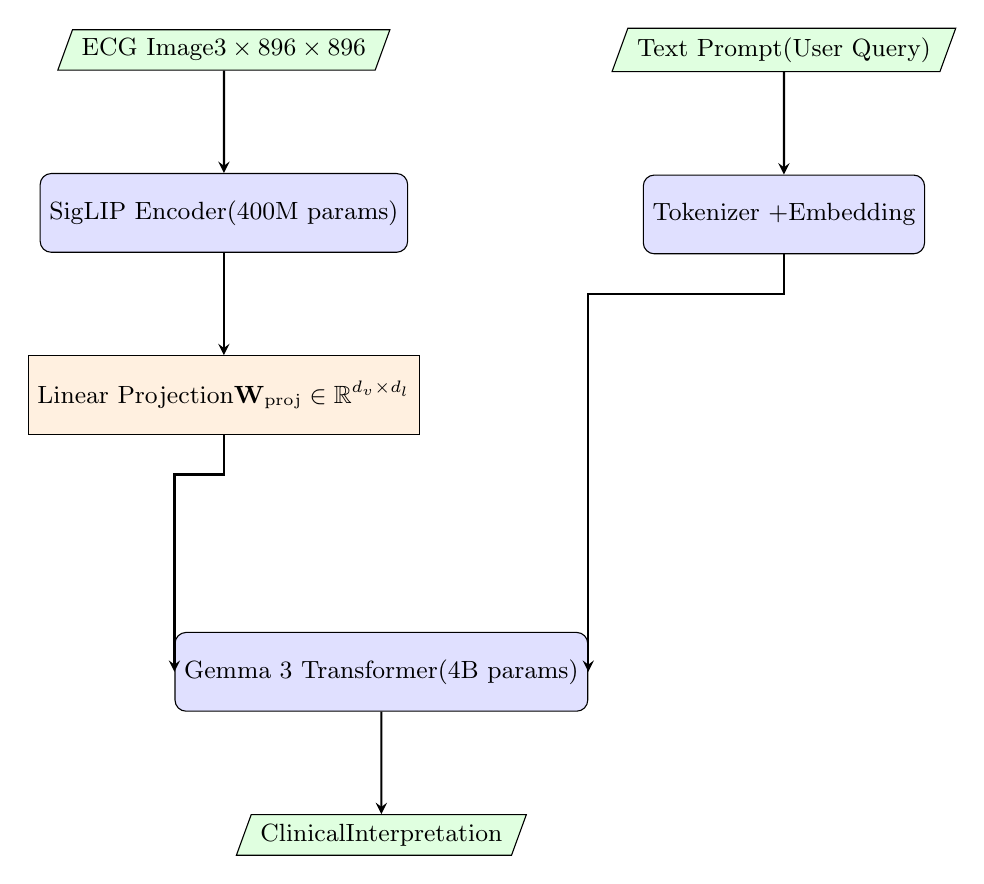
\begin{tikzpicture}[node distance=1.3cm and 2cm, auto]
    \node[data] (img) {ECG Image\\$3 \times 896 \times 896$};
    \node[block, below=of img] (siglip) {SigLIP Encoder\\(400M params)};
    \node[process, below=of siglip] (proj) {Linear Projection\\$\mathbf{W}_{\text{proj}} \in \mathbb{R}^{d_v \times d_l}$};
    \node[data, right=3cm of img] (text) {Text Prompt\\(User Query)};
    \node[block, below=of text] (tok) {Tokenizer +\\Embedding};
    \node[block, below=2.5cm of proj, xshift=2cm] (gemma) {Gemma 3 Transformer\\(4B params)};
    \node[data, below=of gemma] (out) {Clinical\\Interpretation};

    \draw[arrow] (img) -- (siglip);
    \draw[arrow] (siglip) -- (proj);
    \draw[arrow] (proj.south) -- ++(0,-0.5) -| (gemma.west);
    \draw[arrow] (text) -- (tok);
    \draw[arrow] (tok.south) -- ++(0,-0.5) -| (gemma.east);
    \draw[arrow] (gemma) -- (out);
\end{tikzpicture}
\caption{MedGemma multimodal architecture. The SigLIP vision encoder and text embeddings are projected into a shared space and processed by the Gemma~3 transformer.}
\label{fig:architecture}
\end{figure}

% ============================================================
% 3. DATASET
% ============================================================
\section{Dataset}

The first part in building such a system is ofcourse to fine-tune the model on a large corpus of ECG images along with instructions. We chose the PULSE-ECG/ECGInstruct dataset, which contains around 1 million ECG instruction-following samples. It is a composite dataset that consolidates multiple major ECG databases:

\begin{table}[H]
\centering
\caption{Constituent datasets within ECGInstruct}
\begin{tabular}{@{}llp{6cm}@{}}
\toprule
\textbf{Dataset} & \textbf{Samples} & \textbf{Task Type} \\
\midrule
PTB-XL & $\sim$21,000 recordings & 12-lead diagnostic classification with structured labels \\
ECG-QA & $\sim$700,000+ & Visual question-answering over ECG waveforms \\
MIMIC-IV-ECG & $\sim$800,000+ & Multi-label diagnosis from clinical settings \\
CODE-15 & $\sim$345,000 & 15-class arrhythmia classification \\
\bottomrule
\end{tabular}
\end{table}

Each sample follows a conversation format: a ``human'' turn with an ECG image and a question about it, and a ``gpt'' turn with the expert interpretation. This instruction-following format is critical because it trains the model to \textit{explain} what it sees, not just classify. For our fine-tuning we filtered exclusively for the PTB-XL subset, which has the highest-quality clinical annotations with SCP diagnostic codes mapped to human-readable interpretations.

% ============================================================
% 4. FINE-TUNING
% ============================================================
\section{Fine-Tuning}

\subsection{Compute Infrastructure}

We needed at least 8$\times$A100 40GB VRAM GPUs to train this model. We can not fine-tune even the 4B model on 2$\times$T4 or a single P100 from Kaggle, or a single H100 from Colab. The C-DAC AI Innovation Challenge (AIRAWAT AI Innovation Challenge) gave us access to India's AIRAWAT supercomputer with 8$\times$A100-SXM4 GPUs for 7 days. Multi-GPU distribution was handled via \texttt{torchrun} with NCCL backend and DeepSpeed ZeRO Stage~3 for optimizer and parameter sharding across all 8 GPUs.

\subsection{LoRA: Low-Rank Adaptation}

Fine-tuning all 4 billion parameters is infeasible even on 8$\times$A100s when accounting for optimizer states and gradients. We used LoRA (Low-Rank Adaptation), which freezes the original weight matrices and injects trainable low-rank decomposition matrices.

For a pretrained weight matrix $\mathbf{W}_0 \in \mathbb{R}^{d \times k}$, LoRA parameterises the update as:

\begin{equation}
    \mathbf{W} = \mathbf{W}_0 + \Delta\mathbf{W} = \mathbf{W}_0 + \mathbf{B}\mathbf{A}
\end{equation}

where $\mathbf{B} \in \mathbb{R}^{d \times r}$, $\mathbf{A} \in \mathbb{R}^{r \times k}$, and $r \ll \min(d, k)$ is the rank. The forward pass becomes:

\begin{equation}
    h = \mathbf{W}_0 x + \frac{\alpha}{r} \mathbf{B}\mathbf{A}x
\end{equation}

where $\alpha$ is the LoRA scaling factor. Only $\mathbf{A}$ and $\mathbf{B}$ are trained; $\mathbf{W}_0$ remains frozen. This reduces trainable parameters from billions to millions while preserving the model's pre-trained knowledge.

We applied LoRA to \textbf{all linear layers} in the transformer (not just the attention layers, but also the MLP projections), which gives better performance than targeting only Q/K/V projections.

\subsection{Training Configuration}

\begin{table}[H]
\centering
\caption{Fine-tuning hyperparameters}
\begin{tabular}{@{}ll@{}}
\toprule
\textbf{Parameter} & \textbf{Value} \\
\midrule
Base Model & google/medgemma-4b-it \\
LoRA Rank $r$ & 32 \\
LoRA Alpha $\alpha$ & 64 \\
LoRA Dropout & 0.05 \\
LoRA Target & All linear layers \\
Learning Rate & $1.2 \times 10^{-5}$ \\
LR Scheduler & Cosine decay \\
Warmup Ratio & 0.1 \\
Weight Decay & 0.005 \\
Epochs & 3 \\
Per-GPU Batch Size & 4 \\
Gradient Accumulation & 8 steps \\
\textbf{Effective Batch Size} & $\mathbf{4 \times 8 \times 8 = 256}$ \\
Max Sequence Length & 2048 tokens \\
Precision & BF16 \\
Optimizer & AdamW (fused) \\
Max Gradient Norm & 1.0 \\
Parallelism & DeepSpeed ZeRO-3 \\
\bottomrule
\end{tabular}
\end{table}

The effective batch size of 256 is calculated as per-device batch size (4) multiplied by gradient accumulation steps (8) multiplied by the number of GPUs (8). The cosine learning rate schedule with 10\% warmup ensures a gentle start followed by smooth decay, which is important for LoRA fine-tuning where aggressive updates early on can destroy the adapter's alignment with the frozen weights.

\subsection{Loss Function}

We used the standard causal language modelling loss (cross-entropy over next-token prediction). For a sequence of tokens $(x_1, x_2, \ldots, x_n)$, the loss is:

\begin{equation}
    \mathcal{L} = -\frac{1}{N} \sum_{t=1}^{N} \log P_\theta(x_t \mid x_1, \ldots, x_{t-1})
\end{equation}

where $P_\theta$ is the model's predicted probability distribution. Padding tokens, image tokens, and special tokens are masked with label $-100$ so they do not contribute to the loss. Only the ``assistant'' portion of each conversation (the ECG interpretation) is trained on. This is important: we do not want the model to learn to generate user questions, only expert answers.

\subsection{Training Results and Evaluation}

\begin{table}[H]
\centering
\caption{Final training metrics after 3 days on 8$\times$A100}
\begin{tabular}{@{}ll@{}}
\toprule
\textbf{Metric} & \textbf{Value} \\
\midrule
Initial Loss & 9.5907 \\
Final Training Loss & 0.6188 \\
Minimum Loss Achieved & 0.5767 \\
Token Accuracy (Train) & 86.83\% \\
Token Accuracy (Eval) & 85.96\% \\
Training Throughput & $\sim$9.67 samples/sec \\
Total Tokens Processed & 103M+ \\
Total Steps & 102 \\
Final Epoch & 0.91 \\
Mean Gradient Norm & 1.3548 \\
Max Gradient Norm & 6.5353 \\
\bottomrule
\end{tabular}
\end{table}

\begin{figure}[H]
    \centering
    \includegraphics[width=0.95\textwidth]{training_dashboard.png}
    \caption{MedGemma ECG training dashboard. \textbf{Top-left:} Training loss dropped from 9.59 to 0.62 with smooth convergence. \textbf{Top-center:} Token accuracy stabilised at 86.83\% (train) and 85.96\% (eval). \textbf{Top-right:} Cosine learning rate schedule with warmup. \textbf{Bottom-left:} Gradient norms remained stable below 2.0 after initial spike. \textbf{Bottom-right:} Entropy collapsed early (model became confident) and stabilised.}
    \label{fig:training}
\end{figure}

The 86.83\% token accuracy is strong. The train-eval accuracy gap of less than 1\% (86.83\% vs 85.96\%) indicates minimal overfitting, which validates our choice of LoRA rank and dropout. The loss curve in Figure~\ref{fig:training} shows smooth convergence without spikes, meaning the gradient clipping ($\|\nabla\| \leq 1.0$) and learning rate were well-tuned.

The gradient norm plot shows an initial spike to 6.53 (expected when the randomly initialised LoRA adapters first encounter the training signal) followed by rapid stabilisation around 1.35. The entropy plot shows the output distribution becoming sharply peaked within the first 20\% of training. This means the model quickly learns the structured output format and becomes confident in its token predictions.

After training, the LoRA adapters were merged into the base model weights to produce a single checkpoint, uploaded as \texttt{convaiinnovations/medgemma-4b-ecginstruct}.

% Training Pipeline Diagram
\begin{figure}[H]
\centering
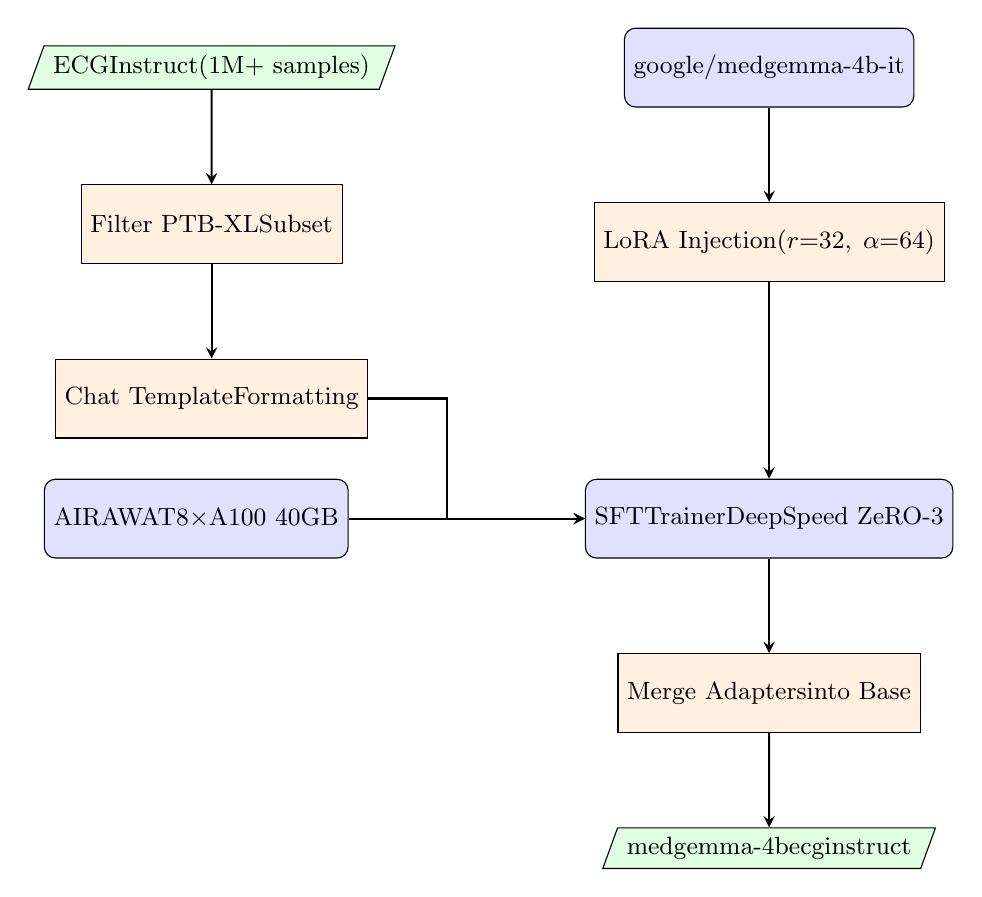
\begin{tikzpicture}[node distance=1.2cm and 1.5cm, auto]
    \node[data] (dataset) {ECGInstruct\\(1M+ samples)};
    \node[process, below=of dataset] (filter) {Filter PTB-XL\\Subset};
    \node[process, below=of filter] (format) {Chat Template\\Formatting};
    \node[block, right=3cm of dataset] (base) {google/\\medgemma-4b-it};
    \node[process, below=of base] (lora) {LoRA Injection\\($r{=}32,\;\alpha{=}64$)};
    \node[block, below=2.5cm of lora] (trainer) {SFTTrainer\\DeepSpeed ZeRO-3};
    \node[process, below=of trainer] (merge) {Merge Adapters\\into Base};
    \node[data, below=of merge] (output) {medgemma-4b\\ecginstruct};
    \node[block, left=3cm of trainer] (hpc) {AIRAWAT\\8$\times$A100 40GB};

    \draw[arrow] (dataset) -- (filter);
    \draw[arrow] (filter) -- (format);
    \draw[arrow] (format.east) -- ++(1cm,0) |- (trainer.west);
    \draw[arrow] (base) -- (lora);
    \draw[arrow] (lora) -- (trainer);
    \draw[arrow] (trainer) -- (merge);
    \draw[arrow] (merge) -- (output);
    \draw[arrow] (hpc) -- (trainer);
\end{tikzpicture}
\caption{End-to-end training pipeline from ECGInstruct to the deployed model.}
\label{fig:training_pipeline}
\end{figure}

% ============================================================
% 5. ONNX VISION ENCODER
% ============================================================
\section{Vision Encoder Extraction and Quantization}

Now comes another problem. We had the fine-tuned LLM, but how do we make an attention heatmap? The \texttt{mmproj} GGUF file projects images into the LLM embedding space during inference, but it does not expose intermediate attention weights. We need to extract the SigLIP vision encoder separately, bundle it with the projection matrix, and export it to a format that can run independently in the desktop app.

We discovered that ONNX Runtime has a Node.js package (\texttt{onnxruntime-node}), so we can run the vision encoder in JavaScript. The conversion was done on Kaggle.

\subsection{Extraction Process}

We loaded the full fine-tuned model in FP16 and extracted two components: the SigLIP vision tower (the backbone that processes image patches) and the multimodal projector weight matrix $\mathbf{W}_{\text{proj}}$. A custom wrapper class bundles these together and adds attention score computation as an additional output head.

The wrapper takes raw pixel values and produces three outputs:
\begin{enumerate}
    \item \textbf{Projected Embeddings} $\mathbf{P} \in \mathbb{R}^{256 \times d_l}$, the patch embeddings mapped into the language model space
    \item \textbf{Attention Scores} $\mathbf{a} \in \mathbb{R}^{256}$, a per-patch importance score
    \item \textbf{Pooled Embedding} $\mathbf{p} \in \mathbb{R}^{d_l}$, a single global image representation
\end{enumerate}

\subsection{Quantization}

The exported FP32 ONNX model was approximately 600\,MB. We applied dynamic quantization (weights quantised to UINT8, activations remain FP32) using ONNX Runtime's built-in quantisation toolkit. This reduced the model to approximately 150\,MB, a 4$\times$ reduction, while preserving inference quality. Dynamic quantisation works well here because the computations are dominated by matrix multiplications where weight quantisation introduces minimal error.

% ONNX Pipeline Diagram
\begin{figure}[H]
\centering
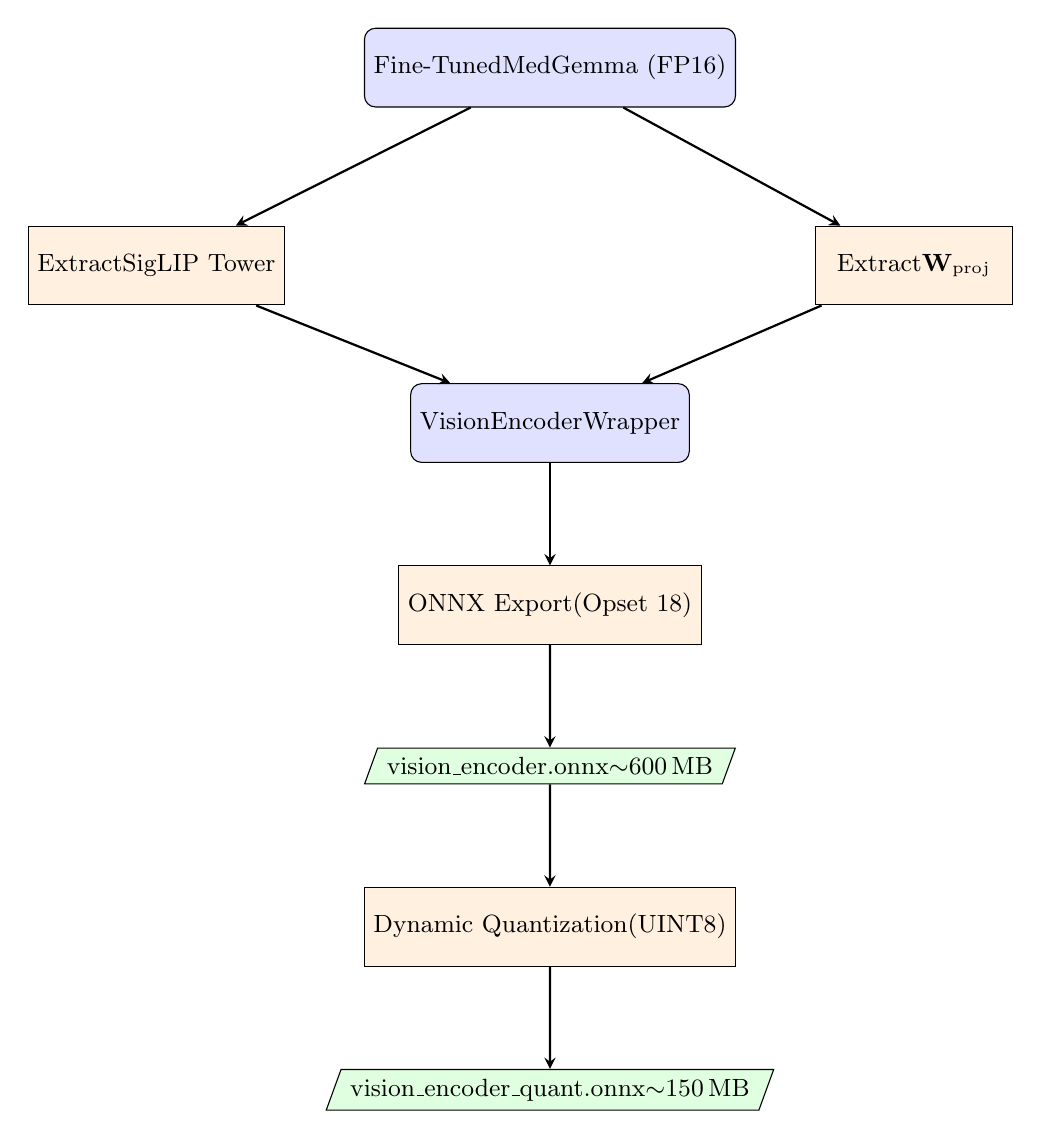
\begin{tikzpicture}[node distance=1.3cm, auto]
    \node[block] (model) {Fine-Tuned\\MedGemma (FP16)};
    \node[process, below left=1.5cm and 1cm of model] (vt) {Extract\\SigLIP Tower};
    \node[process, below right=1.5cm and 1cm of model] (proj) {Extract\\$\mathbf{W}_{\text{proj}}$};
    \node[block, below=3.5cm of model] (wrapper) {VisionEncoder\\Wrapper};
    \node[process, below=of wrapper] (export) {ONNX Export\\(Opset 18)};
    \node[data, below=of export] (fp32) {vision\_encoder.onnx\\$\sim$600\,MB};
    \node[process, below=of fp32] (quant) {Dynamic Quantization\\(UINT8)};
    \node[data, below=of quant] (int8) {vision\_encoder\_quant.onnx\\$\sim$150\,MB};

    \draw[arrow] (model) -- (vt);
    \draw[arrow] (model) -- (proj);
    \draw[arrow] (vt) -- (wrapper);
    \draw[arrow] (proj) -- (wrapper);
    \draw[arrow] (wrapper) -- (export);
    \draw[arrow] (export) -- (fp32);
    \draw[arrow] (fp32) -- (quant);
    \draw[arrow] (quant) -- (int8);
\end{tikzpicture}
\caption{ONNX conversion pipeline: from the full model to a quantised edge-deployable encoder.}
\label{fig:onnx_pipeline}
\end{figure}

% ============================================================
% 6. ATTENTION HEATMAP MATHEMATICS
% ============================================================
\section{Attention Heatmap: Mathematical Foundation}

The heatmap generation is grounded in the mathematical properties of the vision transformer's projection space. The core intuition is that if a region of the ECG image projects into the language model's embedding space with a large magnitude, that region carries significant information for clinical reasoning. This is not just a visualisation trick. It is a direct measurement of how much each image patch contributes to the model's representation.

\subsection{Image Tokenisation and Patch Embedding}

The SigLIP encoder partitions the input image $I \in \mathbb{R}^{3 \times H \times H}$ (where $H = 896$) into a regular grid of non-overlapping patches. Each patch $p_{ij}$ has spatial dimensions $(H/S) \times (H/S)$ where $S$ is the grid side length. The encoder's transformer layers process these patches through $L$ self-attention layers, producing contextualised patch embeddings:

\begin{equation}
    \mathbf{E} = \text{SigLIP}(I) = \{e_1, e_2, \ldots, e_N\}, \quad e_i \in \mathbb{R}^{d_v}
\end{equation}

where $N = S^2$ is the total number of patches and $d_v$ is the vision hidden dimension. Each embedding $e_i$ encodes not just the local patch content but also its relationship with all other patches through the self-attention layers.

\subsection{Spatial Average Pooling}

When $N > 256$ (which happens with high-resolution inputs), we reduce to a fixed $16 \times 16$ grid through spatial average pooling. The embeddings are first reshaped into their 2D spatial layout:

\begin{equation}
    \mathbf{E}_{\text{2D}} \in \mathbb{R}^{S \times S \times d_v}
\end{equation}

Then grouped into $16 \times 16$ superpatches, each containing $k \times k$ original patches where $k = S/16$:

\begin{equation}
    \bar{e}_{ij} = \frac{1}{k^2} \sum_{m=0}^{k-1} \sum_{n=0}^{k-1} e_{(i \cdot k + m),\; (j \cdot k + n)}, \quad i,j \in \{0, \ldots, 15\}
\end{equation}

This yields the pooled embedding matrix $\bar{\mathbf{E}} \in \mathbb{R}^{256 \times d_v}$.

\subsection{Projection into Language Model Space}

The pooled vision embeddings are linearly projected into the language model's token embedding space using the multimodal projector:

\begin{equation}
    \mathbf{P} = \bar{\mathbf{E}} \cdot \mathbf{W}_{\text{proj}}, \quad \mathbf{P} \in \mathbb{R}^{256 \times d_l}
\end{equation}

Each row $\mathbf{P}_i \in \mathbb{R}^{d_l}$ represents how patch $i$ appears in the language model's embedding space. A patch containing a critical ST elevation will have a strong projection, while a blank background patch will project to a near-zero vector.

\subsection{Attention Score: Projection Magnitude}

The attention score for each patch is defined as the L2 norm (Euclidean magnitude) of its projected embedding:

\begin{equation}
    a_i = \|\mathbf{P}_i\|_2 = \sqrt{\sum_{j=1}^{d_l} P_{ij}^2}
\end{equation}

The justification: in the model's embedding space, tokens that carry more meaning tend to have larger norms. This is a known property of transformer embeddings. By computing the norm of the projected visual patch, we are measuring how much that patch contributes when it enters the language model for reasoning.

\subsection{Normalisation}

Raw attention scores are normalised to $[0, 1]$ using Min-Max scaling:

\begin{equation}
    \hat{a}_i = \frac{a_i - a_{\min}}{a_{\max} - a_{\min} + \epsilon}
\end{equation}

where $a_{\min} = \min_i(a_i)$, $a_{\max} = \max_i(a_i)$, and $\epsilon = 10^{-8}$ prevents division by zero.

\subsection{Contrast Enhancement via Linear Windowing}

The normalised scores tend to cluster in a narrow range, making it difficult to visually distinguish important regions from background. We apply a linear windowing function with empirically tuned thresholds:

\begin{equation}
    \tilde{a}_i = \text{clip}\left(\frac{\hat{a}_i - v_{\min}}{v_{\max} - v_{\min}}, \; 0, \; 1\right)
\end{equation}

where $v_{\min} = 0.3$ and $v_{\max} = 0.7$. The clip function is defined as:

\begin{equation}
    \text{clip}(x, 0, 1) = \max(0, \min(1, x))
\end{equation}

This windowing has two key effects:
\begin{itemize}
    \item \textbf{Background suppression:} Any attention below $v_{\min}$ is mapped to 0 (rendered as blue/transparent), eliminating low-level noise from non-diagnostic regions.
    \item \textbf{Signal amplification:} Attention values between $v_{\min}$ and $v_{\max}$ are stretched across the full $[0, 1]$ range, making clinically relevant but subtle signals more visible.
\end{itemize}

\subsection{Colormap Application and Alpha Blending}

The $16 \times 16$ attention grid $\tilde{\mathbf{A}} = [\tilde{a}_1, \ldots, \tilde{a}_{256}]$ reshaped into a $16 \times 16$ matrix is upscaled to the original image resolution using bicubic interpolation. This produces smooth, cloud-like contours rather than a blocky pixelated grid.

A Jet colormap maps scalar attention to RGB:

\begin{equation}
    f_{\text{jet}}: [0, 1] \to \mathbb{R}^3, \quad
    \tilde{a}_i \mapsto \begin{cases}
    (0, 0, 1) & \text{(Blue)} \quad \tilde{a}_i \to 0 \\
    (1, 1, 0) & \text{(Yellow)} \quad \tilde{a}_i \approx 0.5 \\
    (1, 0, 0) & \text{(Red)} \quad \tilde{a}_i \to 1
    \end{cases}
\end{equation}

The final overlay uses alpha blending:

\begin{equation}
    I_{\text{overlay}}(x,y) = (1 - \alpha) \cdot I_{\text{original}}(x,y) + \alpha \cdot I_{\text{heatmap}}(x,y)
\end{equation}

with $\alpha = 0.5$. Low-attention regions (blue) are set to fully transparent ($\alpha = 0$) so the original ECG trace remains clearly visible underneath.

% Attention Pipeline Diagram
\begin{figure}[H]
\centering
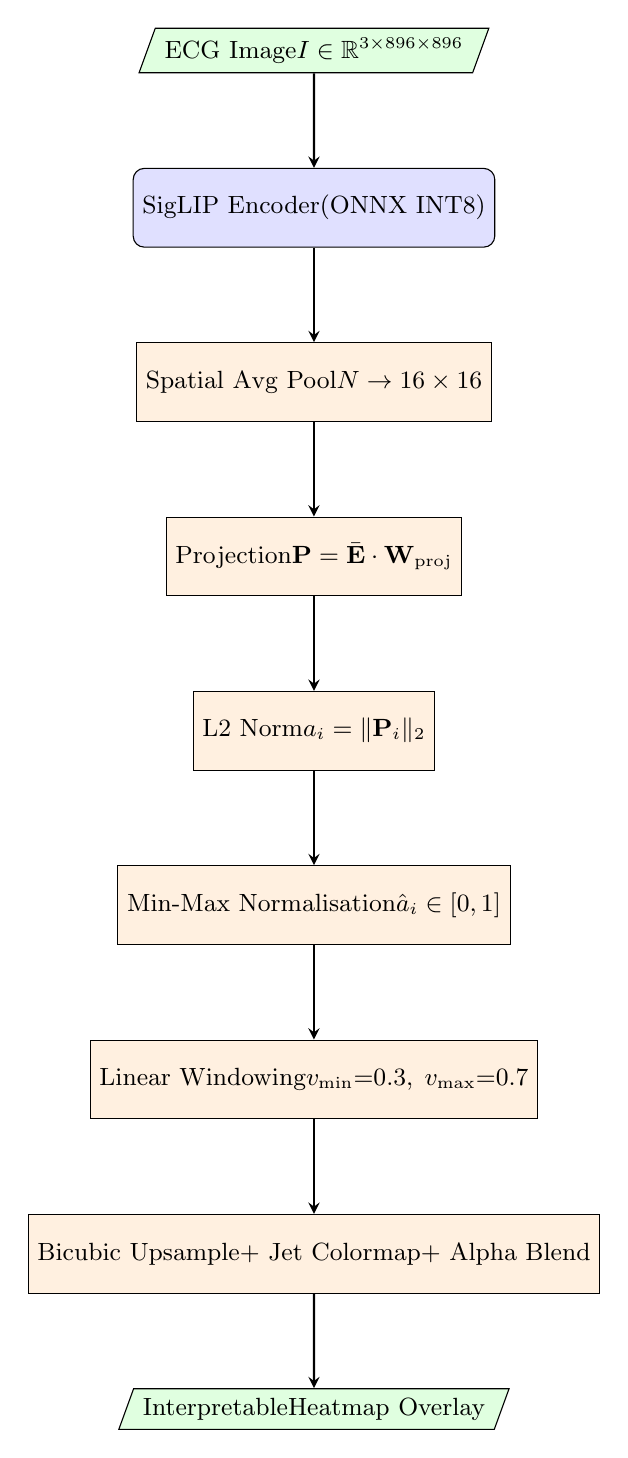
\begin{tikzpicture}[node distance=1.2cm, auto]
    \node[data] (ecg) {ECG Image\\$I \in \mathbb{R}^{3 \times 896 \times 896}$};
    \node[block, below=of ecg] (siglip) {SigLIP Encoder\\(ONNX INT8)};
    \node[process, below=of siglip] (pool) {Spatial Avg Pool\\$N \to 16 \times 16$};
    \node[process, below=of pool] (proj) {Projection\\$\mathbf{P} = \bar{\mathbf{E}} \cdot \mathbf{W}_{\text{proj}}$};
    \node[process, below=of proj] (norm) {L2 Norm\\$a_i = \|\mathbf{P}_i\|_2$};
    \node[process, below=of norm] (minmax) {Min-Max Normalisation\\$\hat{a}_i \in [0,1]$};
    \node[process, below=of minmax] (window) {Linear Windowing\\$v_{\min}{=}0.3,\; v_{\max}{=}0.7$};
    \node[process, below=of window] (render) {Bicubic Upsample\\+ Jet Colormap\\+ Alpha Blend};
    \node[data, below=of render] (heatmap) {Interpretable\\Heatmap Overlay};

    \draw[arrow] (ecg) -- (siglip);
    \draw[arrow] (siglip) -- (pool);
    \draw[arrow] (pool) -- (proj);
    \draw[arrow] (proj) -- (norm);
    \draw[arrow] (norm) -- (minmax);
    \draw[arrow] (minmax) -- (window);
    \draw[arrow] (window) -- (render);
    \draw[arrow] (render) -- (heatmap);
\end{tikzpicture}
\caption{Complete attention heatmap pipeline from raw ECG image to interpretable overlay.}
\label{fig:attention_pipeline}
\end{figure}

\subsection{Clinical Interpretability}

This system allows clinicians to verify \textit{why} the AI made a particular diagnosis. If the model predicts ``Anterior STEMI'', the heatmap should glow red over the ST-segments in leads V3 and V4. If the model predicts a condition but the heatmap highlights an artifact, a movement artefact, or empty background, the clinician can immediately dismiss the result as unreliable. This is the key value: we are not asking doctors to trust the AI blindly, we are giving them a tool to verify the AI's reasoning.

% ============================================================
% 7. LANGGRAPH ORCHESTRATION
% ============================================================
\section{Agentic Orchestration with LangGraph}

This is the most important architectural decision we made for the desktop application. The main problem is that we are uploading an ECG image \textit{and} a blood report, both of which need to be analysed and combined to get a final diagnosis. Additionally, we need to integrate the ONNX vision encoder for heatmap generation. A simple sequential pipeline does not work because ECG analysis and PDF parsing are independent and should run in parallel, the synthesis step needs results from both, sometimes the user only uploads one of the two, and we also need a general chat mode.

We chose LangGraph JS and designed a stateful directed graph with five functional nodes and conditional routing.

\subsection{State Graph Formalism}

The agent maintains a shared state $\mathcal{S}$ that flows through the graph. Each node is a function $f_i: \mathcal{S} \to \Delta\mathcal{S}$ that reads the current state and returns a partial update. Updates are merged using reducers. The \texttt{messages} field uses an append reducer (conversation only grows, never shrinks), while all other fields use a last-write-wins reducer.

\begin{table}[H]
\centering
\caption{Agent state schema $\mathcal{S}$}
\begin{tabular}{@{}llp{6cm}@{}}
\toprule
\textbf{Field} & \textbf{Type} & \textbf{Semantics} \\
\midrule
\texttt{messages} & List & Full conversation history (append-only) \\
\texttt{ecgFindings} & Text & ECG analysis from the model \\
\texttt{ecgPath} & Text & File path to the uploaded ECG image \\
\texttt{reportFindings} & Text & Extracted clinical report context \\
\texttt{heatmapPath} & Text & Path to the generated heatmap \\
\texttt{clinicalAssessment} & Text & Combined clinical assessment \\
\texttt{nextSteps} & List & Recommended next steps \\
\texttt{lifestyleRecommendations} & List & Lifestyle modifications \\
\bottomrule
\end{tabular}
\end{table}

\subsection{Node Descriptions}

\textbf{Router Node} inspects the incoming message for file markers (\texttt{[ECG:~...]} and \texttt{[Report:~...]}) and returns the set of downstream nodes to activate. When both markers are present, it returns a list, triggering parallel execution of both branches.

\textbf{ECG Node} delegates the image to the Vision Worker thread (running the ONNX encoder), which generates the heatmap overlay and returns the heatmap file path. The original ECG path is also stored in state for the synthesis node to pass to the multimodal LLM.

\textbf{PDF Node} reads the uploaded PDF, extracts all text, and sends it to a RAG (Retrieval-Augmented Generation) worker. The RAG worker chunks the text, computes embeddings, and retrieves the chunks most semantically relevant to the user's query using cosine similarity.

\textbf{Synthesis Node} is the core reasoning engine. It takes the ECG image path and the PDF-extracted context, constructs a clinical prompt, and passes everything to the MedGemma LLM via the multimodal projector. The LLM receives the ECG image as visual tokens and generates a structured clinical assessment with four sections: ECG Analysis, Assessment, Next Steps, and Lifestyle Recommendations.

\textbf{Chat Node} handles general conversational queries when no files are attached.

\subsection{Graph Topology}

The graph has the following edge structure:

\begin{itemize}
    \item $\text{START} \to \text{Router}$
    \item $\text{Router} \xrightarrow{\text{conditional}} \{\text{ECG}, \text{PDF}, \text{Chat}\}$ (parallel when both present)
    \item $\text{ECG} \to \text{Synthesis}$
    \item $\text{PDF} \to \text{Synthesis}$ (both converge here)
    \item $\text{Synthesis} \to \text{END}$
    \item $\text{Chat} \to \text{END}$
\end{itemize}

When both ECG and PDF are present, the router triggers parallel execution. LangGraph waits for all upstream nodes to complete before running the synthesis node.

% LangGraph Diagram
\begin{figure}[H]
\centering
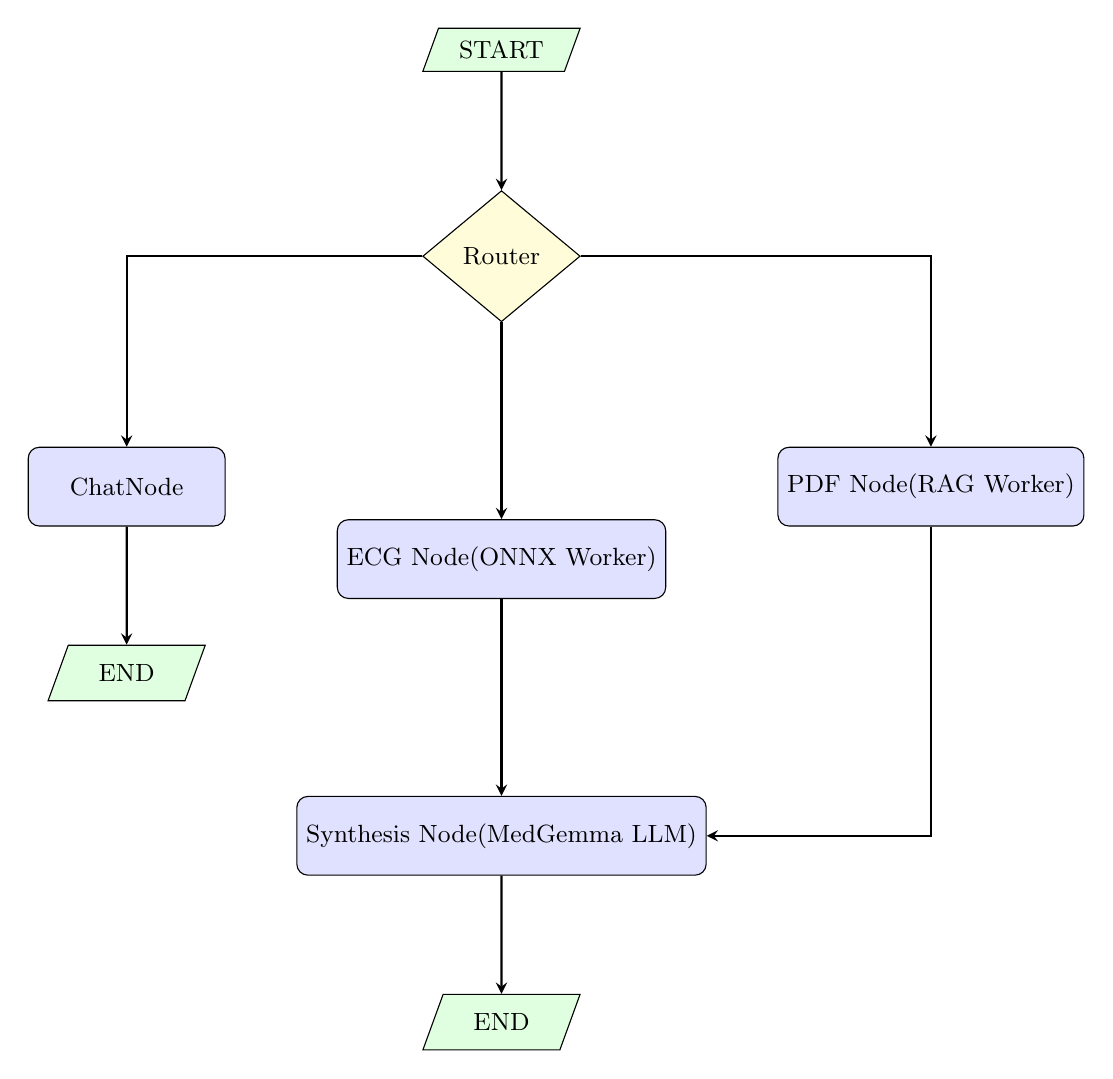
\begin{tikzpicture}[node distance=1.5cm and 2.5cm, auto]
    \node[data] (start) {START};
    \node[decision, below=of start] (router) {Router};

    \node[block, below left=2cm and 3cm of router] (chat) {Chat\\Node};
    \node[block, below=2.5cm of router] (ecg) {ECG Node\\(ONNX Worker)};
    \node[block, below right=2cm and 3cm of router] (pdf) {PDF Node\\(RAG Worker)};

    \node[block, below=2.5cm of ecg] (synth) {Synthesis Node\\(MedGemma LLM)};

    \node[data, below=of synth] (endnode) {END};
    \node[data, below=1.5cm of chat] (chatend) {END};

    \draw[arrow] (start) -- (router);
    \draw[arrow] (router) -| (chat);
    \draw[arrow] (router) -- (ecg);
    \draw[arrow] (router) -| (pdf);
    \draw[arrow] (ecg) -- (synth);
    \draw[arrow] (pdf) |- (synth);
    \draw[arrow] (synth) -- (endnode);
    \draw[arrow] (chat) -- (chatend);
\end{tikzpicture}
\caption{LangGraph state graph topology. The router conditionally dispatches to ECG and/or PDF nodes (parallel when both present), which converge at the Synthesis node for combined reasoning.}
\label{fig:langgraph}
\end{figure}

\subsection{Worker Thread Isolation}

Both the ONNX vision encoder and the RAG retrieval system run in separate Node.js Worker Threads. This is needed because ONNX inference and PDF parsing are CPU-intensive operations that would freeze the UI if run on the main thread. The workers are initialised once during application startup and communicate with the agent via message passing.

% ============================================================
% 8. SYSTEM OVERVIEW
% ============================================================
\section{System Overview}

The complete system uses three model files stored locally:
\begin{itemize}
    \item \texttt{ggml-model-q4\_k\_m.gguf}, the Q4\_K\_M quantised MedGemma LLM ($\sim$2.5\,GB)
    \item \texttt{mmproj-medgemma-4b-ecginstruct-F16.gguf}, multimodal projector in FP16
    \item \texttt{vision\_encoder\_quant.onnx}, INT8 quantised SigLIP encoder ($\sim$150\,MB)
\end{itemize}

The LLM is served via \texttt{node-llama-cpp}, the vision encoder via \texttt{onnxruntime-node}, and the orchestration via \texttt{@langchain/langgraph}. Everything runs on a single machine with no network dependency. The application is built with Electron and uses SQLite for storing analysis history.

The user uploads an ECG image and/or a blood report PDF, and the system produces: (1) a structured clinical assessment, (2) an attention heatmap highlighting the regions the model focused on, (3) recommended next steps, and (4) lifestyle recommendations. All of this happens locally, and the patient's data never leaves the device.

% ============================================================
% 9. CONCLUSION
% ============================================================
\section{Conclusion}

We have presented AI4Cardio, an offline desktop application that combines a fine-tuned multimodal medical model, an explainable attention heatmap system, and a graph-based orchestration for automated ECG and blood report interpretation. The model was trained on India's AIRAWAT supercomputer using 8$\times$A100 GPUs and achieves 86.83\% token accuracy on ECG interpretation tasks with less than 1\% train-eval gap.

The attention heatmap system provides a mathematically grounded method for clinicians to verify the model's reasoning, based on the projection magnitude of vision patches in the embedding space. The LangGraph orchestration enables parallel processing of multimodal inputs with conditional routing and structured output generation.

Everything runs offline on commodity hardware, making it deployable in resource-constrained clinical settings where internet connectivity and specialist availability are limited.

\vspace{1cm}
\noindent\textbf{Links:}
\begin{itemize}[leftmargin=*]
    \item Desktop App: \href{https://github.com/NandhaKishorM/electron_app_heart}{github.com/NandhaKishorM/electron\_app\_heart}
    \item Fine-Tuned Model: \href{https://huggingface.co/convaiinnovations/medgemma-4b-ecginstruct}{huggingface.co/convaiinnovations/medgemma-4b-ecginstruct}
    \item Training Metrics: \href{https://huggingface.co/convaiinnovations/medgemma-ecg-training-metrics}{huggingface.co/convaiinnovations/medgemma-ecg-training-metrics}
\end{itemize}

\end{document}
